% !TeX root = ../main.tex
% 原始章节：09-cache.Rmd

\chapter{Cache设计}\label{chap:09-cache}

\section{Cache基本结构与原理}\label{sec:09-cache-001}

\subsection{Cache的设计规格}\label{sec:09-cache-002}

为保证流水线的满负荷运转，处理器一般采用哈弗架构，集成一个指令Cache和一个数据Cache。为使读者可以更便捷的理解Cache并构建自己的指令和数据缓存，本文给出了一个可供参考的设计规格，尽管在更复杂的设计中可能采用更复杂的Cache结构，但下面的结构也足以满足学习甚至嵌入式场景的复杂度和性能需求。本文后续的Cache介绍都沿用这个规格。

\subsubsection{Cache结构}\label{sec:09-cache-003}

\begin{enumerate}
\def\labelenumi{\arabic{enumi}.}
\tightlist
\item
  \textbf{Cache容量与结构}：

  \begin{itemize}
  \tightlist
  \item
    指令Cache和数据Cache的容量均为8KB。
  \item
    均为两路组相联。
  \item
    Cache行大小均为16字节，也就是4个字。
  \end{itemize}
\item
  \textbf{访问形式}：

  \begin{itemize}
  \tightlist
  \item
    指令Cache和数据Cache均采用Tag和Data同步访问形式。
  \item
    均采用``虚Index实Tag''（VIPT）访问形式。
  \end{itemize}
\item
  \textbf{替换策略}：

  \begin{itemize}
  \tightlist
  \item
    采用伪随机替换算法。
  \end{itemize}
\item
  \textbf{写策略}：

  \begin{itemize}
  \tightlist
  \item
    数据Cache采用写回写分配策略。
  \end{itemize}
\item
  \textbf{设计特性}：

  \begin{itemize}
  \tightlist
  \item
    采用阻塞式（Blocking）设计，即一旦发生Cache Miss（未命中），则阻塞后续访问直至数据填回Cache中。
  \item
    不采用``关键字优先''技术。
  \end{itemize}
\end{enumerate}

\subsubsection{设计初衷}\label{sec:09-cache-004}

\begin{enumerate}
\def\labelenumi{\arabic{enumi}.}
\tightlist
\item
  \textbf{指令Cache与数据Cache的设置}：

  \begin{itemize}
  \tightlist
  \item
    保证流水线满负荷运转。
  \end{itemize}
\item
  \textbf{Cache规格一致性}：

  \begin{itemize}
  \tightlist
  \item
    规格一致性便于将Cache模块实例化两份，分别实现指令Cache和数据Cache，减轻开发和调试工作量。
  \end{itemize}
\item
  \textbf{两路组相联设计}：

  \begin{itemize}
  \tightlist
  \item
    直接映射设计过于简单，而两路组相联在多路组相联结构中复杂度最低且具有代表性，易于后续调整。
  \end{itemize}
\item
  \textbf{容量与行大小}：

  \begin{itemize}
  \tightlist
  \item
    每一路Cache的容量定义为4KB，以规避VIPT方式下的Cache别名问题。
  \item
    Cache行大小定为16字节，以控制Cache Data部分的分体数目在适中规模，未采用64字节以简化设计。
  \end{itemize}
\item
  \textbf{同步访问形式}：

  \begin{itemize}
  \tightlist
  \item
    采用Tag和Data同步访问形式，降低Cache命中情况下的执行周期数。
  \end{itemize}
\item
  \textbf{VIPT设计}：

  \begin{itemize}
  \tightlist
  \item
    VIPT方式将TLB查找与Cache访问并行进行，提升CPU频率。
  \end{itemize}
\item
  \textbf{替换算法选择}：

  \begin{itemize}
  \tightlist
  \item
    伪随机替换算法简单实用，尽管LRU算法性能更佳，但维护LRU信息复杂度较高。
  \end{itemize}
\item
  \textbf{写策略选择}：

  \begin{itemize}
  \tightlist
  \item
    数据Cache写回写分配策略简化写操作Cache Miss处理流程，与读操作Cache Miss处理流程一致。
  \end{itemize}
\item
  \textbf{阻塞式设计}：

  \begin{itemize}
  \tightlist
  \item
    当前静态顺序执行的流水线设计下，非阻塞式Cache设计不会提升整体性能。
  \end{itemize}
\item
  \textbf{不采用``关键字优先''技术}：

  \begin{itemize}
  \tightlist
  \item
    降低与AXI总线交互的复杂度。
  \end{itemize}
\end{enumerate}

\subsubsection{Cache容量计算}\label{sec:09-cache-005}

Cache缓存容量计算如下：
\[
\text{Cache缓存容量} = \text{路数} \times \text{路大小} = 2 \text{路} \times 4 \text{KB} = 8 \text{KB}
\]

\subsubsection{地址位数计算}\label{sec:09-cache-006}

根据设计规格，地址相关的Tag、Index和Offset的位数计算如下：

\begin{itemize}
\tightlist
\item
  \textbf{Offset}：Cache行内偏移，宽度为log2(Cache行大小)，即4位。
\item
  \textbf{Index}：Cache组索引，宽度为log2(路大小) - 5，即8位。
\item
  \textbf{Tag}：Cache行的Tag域，宽度为物理地址宽度 - log2(路大小)，即20位。
\end{itemize}

\subsubsection{地址访问}\label{sec:09-cache-007}

对Cache进行访问时，使用虚地址{[}31:0{]}中的{[}11:4{]}作为Index索引，使用物理地址的高20位（{[}31:12{]}）作为Tag进行比较。地址划分形式如图\ref{fig:cache-access-address-division}所示。

\begin{figure}[htbp]
  \centering
  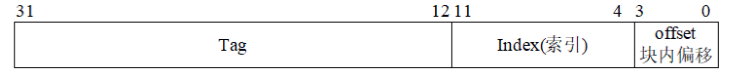
\includegraphics[width=1\linewidth]{assets/09/cache_access_address_division.png}
  \caption{Cache地址划分示意图}
  \label{fig:cache-access-address-division}
\end{figure}

\subsection{Cache模块的数据通路设计}\label{sec:09-cache-008}

\subsubsection{Cache的执行过程}\label{sec:09-cache-009}

\textbf{读操作执行过程}

\begin{itemize}
\item
  \textbf{第一拍}

  \begin{enumerate}
  \def\labelenumi{\arabic{enumi}.}
  \tightlist
  \item
    \textbf{索引值生成}：将请求中虚地址的{[}11:4{]}位作为索引值（index）送往Cache。
  \item
    \textbf{Cache行读取}：将两路Cache中对应同一index的两个Cache行都读出来。
  \item
    \textbf{地址转换}：将读操作的虚地址送往MMU逻辑进行虚实地址转换，物理地址由虚地址的组合逻辑运算结果生成。
  \item
    \textbf{地址寄存}：使用触发器（reg型变量）将物理地址寄存下来，供第二拍使用。
  \end{enumerate}
\item
  \textbf{第二拍}

  \begin{enumerate}
  \def\labelenumi{\arabic{enumi}.}
  \item
    \textbf{Tag信息比较}：

    \begin{itemize}
    \tightlist
    \item
      读取Cache RAM返回的两个Cache行的Tag信息（Cache RAM为单周期返回的同步RAM）。
    \item
      将两个Cache行的Tag信息与锁存下来的物理地址的{[}31:12{]}进行比较。
    \item
      如果某个Cache行的Tag匹配且有效位V等于1，则表示访问命中该Cache行。
    \end{itemize}
  \item
    \textbf{数据选择}：

    \begin{itemize}
    \tightlist
    \item
      根据锁存下来的虚地址的{[}3:2{]}位选择两个Cache行的Data信息，得到访问的32位数据。
    \end{itemize}
  \item
    \textbf{数据返回}：

    \begin{itemize}
    \item
      根据Tag比较结果，将命中的32位数据返回。
    \item
      如果没有命中任何Cache行，则通过总线接口向外发起访存请求，等待访存结果返回Cache模块。
    \item
      从返回结果中取出访问所在的32位数据并返回。
    \end{itemize}
  \end{enumerate}
\end{itemize}

\textbf{写操作执行过程}

\begin{itemize}
\item
  \textbf{第一拍}

  \begin{enumerate}
  \def\labelenumi{\arabic{enumi}.}
  \tightlist
  \item
    \textbf{索引值生成}：将请求中虚地址的{[}11:4{]}位作为索引值（index）送往Cache。
  \item
    \textbf{Tag信息读取}：将两路Cache中对应同一index的两个Cache行的Tag和有效位V信息读出来。
  \item
    \textbf{地址转换}：将写操作的虚地址送往MMU逻辑进行虚实地址转换，物理地址由虚地址的组合逻辑运算结果生成。
  \item
    \textbf{地址寄存}：使用触发器（reg型变量）将物理地址寄存下来，供第二拍使用。
  \end{enumerate}
\item
  \textbf{第二拍}

  \begin{enumerate}
  \def\labelenumi{\arabic{enumi}.}
  \tightlist
  \item
    \textbf{Tag信息比较}：

    \begin{itemize}
    \tightlist
    \item
      读取Cache RAM返回的两个Cache行的Tag信息（Cache RAM为单周期返回的同步RAM）。
    \item
      将两个Cache行的Tag信息与锁存下来的物理地址的{[}31:12{]}进行比较。
    \item
      如果某个Cache行的Tag匹配且有效位V等于1，则表示访问命中该Cache行。
    \end{itemize}
  \item
    \textbf{写操作准备}：

    \begin{itemize}
    \tightlist
    \item
      生成要写入的Index、路号、offset、写使能信号（写32位数据里的哪些字节）。
    \item
      将写数据传入Write Buffer。
    \end{itemize}
  \item
    \textbf{数据写入}：

    \begin{itemize}
    \tightlist
    \item
      如果Cache命中：由Write Buffer向Cache发出写请求，将Write Buffer中缓存的数据写入命中的Cache行的对应位置，并将该Cache行的脏位D置为1。
    \item
      如果Cache缺失：发起访存请求，等待访存结果返回Cache模块后，将store操作待写入的数据和访存结果拼合在一起，一并写入Cache中。
    \end{itemize}
  \end{enumerate}
\end{itemize}

\textbf{Cache缺失处理}

读、写操作都涉及Cache缺失情况下的处理，具体步骤如下：

\begin{enumerate}
\def\labelenumi{\arabic{enumi}.}
\tightlist
\item
  将Cache缺失的地址以及操作类型（如果是写操作，还要记录写数据）记录下来。
\item
  通过AXI总线接口模块向外发起对缺失Cache行的访问。访问地址是缺失Cache行的起始地址，大小是一个Cache行的大小。
\item
  在等待读请求数据返回的过程中（或同时），根据替换算法从Cache Miss地址对应index的两个Cache行中选择一个，将其整个读出。如果该Cache行的V=1且D=1，意味着这是一个有有效脏数据的Cache行，需要将该Cache行的数据通过AXI总线接口模块写出去；否则，直接丢弃该Cache行的数据。这一步还要记录选择了哪一路。
\item
  待缺失请求的数据从总线返回后，生成将要填入Cache的Cache行信息，其中Cache行的V置为1，Tag信息来自之前保存的Cache缺失的地址。如果Cache Miss请求是写操作引起的，Cache行的D置为1，Data信息是store操作待写入值部分覆盖总线返回数据后形成的新数据；否则D置为0，Data信息仅来自总线返回的数据。
\item
  将该Cache行信息填入之前记录的那个位置。
\end{enumerate}

\subsubsection{Cache表的组织管理}\label{sec:09-cache-010}

\textbf{Cache结构的表格分解}

根据Cache行中的信息，将原本的一张表拆分成多张表。对于当前实现的Cache规格，有以下表格：

\begin{itemize}
\item 两张256项×20比特的Tag表
\item 两张256项×1比特的V表
\item 两张256项×1比特的D表
\item 两张256项×128比特的Data表
\end{itemize}


每张表对应Cache的一路。Cache第i路的所有表的第i项构成第i路Cache的index=i的Cache行。所有Cache模块的操作落实到这些表上，只有读和写。下面本文将分析每张表需要支持的读写操作以及读写请求的来源。

\textbf{Cache访问类型}

依据读、写操作访问Cache执行过程中所属的不同阶段，对Cache模块进行的访问可以归纳为四种：Look Up、Hit Write、Replace和Refill。以下是这四种访问的定义：

\begin{enumerate}
\def\labelenumi{\arabic{enumi}.}
\tightlist
\item
  \textbf{Look Up}：判断是否命中Cache，并根据命中信息选取Data部分的内容。
\item
  \textbf{Hit Write}：命中的写操作进入Write Buffer，随后将数据写入命中Cache行的对应位置。
\item
  \textbf{Replace}：为了给Refill的数据腾出位置而发起的读取一个Cache行的操作。
\item
  \textbf{Refill}：将内存返回的数据（以及store miss待写入的数据）填入Replace空出的位置。
\end{enumerate}

\textbf{具体表格的读写支持}

\begin{longtable}[]{@{}
  >{\raggedright\arraybackslash}p{(\linewidth - 8\tabcolsep) * \real{0.1241}}
  >{\raggedright\arraybackslash}p{(\linewidth - 8\tabcolsep) * \real{0.1931}}
  >{\raggedright\arraybackslash}p{(\linewidth - 8\tabcolsep) * \real{0.1931}}
  >{\raggedright\arraybackslash}p{(\linewidth - 8\tabcolsep) * \real{0.1793}}
  >{\raggedright\arraybackslash}p{(\linewidth - 8\tabcolsep) * \real{0.3103}}@{}}
\toprule\noalign{}
\begin{minipage}[b]{\linewidth}\raggedright
表格类型
\end{minipage} & \begin{minipage}[b]{\linewidth}\raggedright
Look Up
\end{minipage} & \begin{minipage}[b]{\linewidth}\raggedright
Replace
\end{minipage} & \begin{minipage}[b]{\linewidth}\raggedright
Hit Write
\end{minipage} & \begin{minipage}[b]{\linewidth}\raggedright
Refill
\end{minipage} \\
\midrule\noalign{}
\endhead
\bottomrule\noalign{}
\endlastfoot
\textbf{Tag表} & 读Tag表，进行Tag比较 & 读Tag表，确定被替换行的信息 & - & 写Tag表，更新新的Tag信息 \\
\textbf{V表} (有效位表) & 读V表，判断Cache行是否有效 & 读V表，确定替换行是否有效 & - & 写V表，更新有效位 \\
\textbf{D表} (脏位表) & - & 读D表，判断被替换行是否脏 & 写D表，将命中行的脏位置为1 & 写D表，更新脏位（根据是否为写操作引起的缺失） \\
\textbf{Data表} & 读Data表，选取对应的Data部分 & 读Data表，获取被替换行的数据 & 写Data表，将数据写入命中行 & 写Data表，将新数据填入替换行 \\
\end{longtable}

对于Tag和V表，所有Cache访问的操作是一致的。因此可以将Tag表和V表横向拼接成一张\{Tag, V\}表，规格为256项×21比特，每项的{[}20:1{]}对应Tag信息，{[}0{]}对应V信息。

进一步分析，Replace和Refill不会同时发生，这意味着对所有表格，Replace的读和Refill的写不会同时进行。由于设计的是阻塞式Cache，在进行Replace和Refill操作时不接收新的访问请求，也不会有Cache命中的store操作。因此，Replace和Refill的读写操作不会与Look Up和Hit Write的读写操作同时发生。此外，Hit Write不访问\{Tag, V\}表，因此\{Tag, V\}表同一时刻至多接收一个读请求或写请求；Look Up不访问D表，因此D表同一时刻至多接收一个读请求或写请求。

Data表的情况较复杂，因为Look Up和Hit Write可能同时发生。直接方案是让Data表支持同时读写，但这种设计成本较高。另一方案是阻塞读操作的Look Up，以避免与Hit Write冲突，虽然降低电路开销但牺牲性能。更好的方法是将Data表横向拆分成四个Bank表，每个规格为256项×32比特。这样，当Look Up和Hit Write不冲突时，可以同时进行；如有冲突，则阻塞Look Up。此方法性能损失较少，且Bank表的写粒度需精细到字节，以支持SB、SH等写操作。

根据以上分析，Cache最终需要使用的存储器规格如下：

\begin{longtable}[]{@{}
  >{\raggedright\arraybackslash}p{(\linewidth - 8\tabcolsep) * \real{0.1733}}
  >{\raggedright\arraybackslash}p{(\linewidth - 8\tabcolsep) * \real{0.1600}}
  >{\raggedright\arraybackslash}p{(\linewidth - 8\tabcolsep) * \real{0.1200}}
  >{\raggedright\arraybackslash}p{(\linewidth - 8\tabcolsep) * \real{0.1333}}
  >{\raggedright\arraybackslash}p{(\linewidth - 8\tabcolsep) * \real{0.4133}}@{}}
\toprule\noalign{}
\begin{minipage}[b]{\linewidth}\raggedright
表格名称
\end{minipage} & \begin{minipage}[b]{\linewidth}\raggedright
规格
\end{minipage} & \begin{minipage}[b]{\linewidth}\raggedright
实现方式
\end{minipage} & \begin{minipage}[b]{\linewidth}\raggedright
实例化数量
\end{minipage} & \begin{minipage}[b]{\linewidth}\raggedright
备注
\end{minipage} \\
\midrule\noalign{}
\endhead
\bottomrule\noalign{}
\endlastfoot
\{Tag, V\}表 & 256项×21比特 & Block RAM & 2 & 每项{[}20:1{]}为Tag信息，{[}0{]}为V信息 \\
Data Bank表 & 256项×32比特 & Block RAM & 8 & 支持字节写使能 \\
D表（脏位表） & 256项×1比特 & Regfile & 2 & - \\
\end{longtable}

\subsection{Cache模块功能边界划分}\label{sec:09-cache-011}

\subsubsection{Cache与CPU的交互}\label{sec:09-cache-012}

基于当前的设计要求，我们希望在Cache与CPU流水线之间的功能边界划分上与现有的``类SRAM-AXI''转接桥和CPU流水线之间的功能边界划分保持一致。具体而言，即是由CPU流水线向Cache模块发送请求，而Cache模块则负责向CPU流水线返回数据或确认写入成功的响应。这样划分后，CPU流水线部分基本无需进行改动。

由于我们采用VIPT（Virtually Indexed Physically Tagged）方式进行Cache访问，因此需要CPU中的TLB（Translation Lookaside Buffer）模块将转换后的物理地址传送至Cache模块。Cache模块接收该物理地址并将其寄存一个时钟周期，然后使用该物理地址进行Cache Tag比较。

总结如下：

\begin{enumerate}
\item \textbf{功能边界划分}：
\begin{itemize}
\item CPU流水线发送请求至Cache模块。
\item Cache模块返回数据或写成功响应至CPU流水线。
\end{itemize}
\end{enumerate}


\begin{enumerate}
\def\labelenumi{\arabic{enumi}.}
\setcounter{enumi}{1}
\tightlist
\item
  \textbf{VIPT Cache访问}：

  \begin{itemize}
  \tightlist
  \item
    TLB模块在CPU中进行虚拟地址到物理地址的转换。
  \item
    转换后的物理地址传送至Cache模块。
  \item
    Cache模块将物理地址寄存一个时钟周期用于Tag比较。
  \end{itemize}
\end{enumerate}

以下是一个可能的Cache模块与CPU流水线的交互接口定义：

\begin{longtable}[]{@{}
  >{\raggedright\arraybackslash}p{(\linewidth - 6\tabcolsep) * \real{0.0933}}
  >{\raggedright\arraybackslash}p{(\linewidth - 6\tabcolsep) * \real{0.0533}}
  >{\raggedright\arraybackslash}p{(\linewidth - 6\tabcolsep) * \real{0.0533}}
  >{\raggedright\arraybackslash}p{(\linewidth - 6\tabcolsep) * \real{0.8000}}@{}}
\toprule\noalign{}
\begin{minipage}[b]{\linewidth}\raggedright
名称
\end{minipage} & \begin{minipage}[b]{\linewidth}\raggedright
位宽
\end{minipage} & \begin{minipage}[b]{\linewidth}\raggedright
方向
\end{minipage} & \begin{minipage}[b]{\linewidth}\raggedright
含义
\end{minipage} \\
\midrule\noalign{}
\endhead
\bottomrule\noalign{}
\endlastfoot
valid & 1 & IN & 表明请求有效 \\
op & 1 & IN & 1：WRITE；0：READ \\
index & 8 & IN & 地址的index域(addr{[}11:4{]}) \\
tag & 20 & IN & 经虚实地址转换后的paddr形成的tag，由于来自组合逻辑运算，故与index是同拍信号。 \\
offset & 4 & IN & 地址的offset域(addr{[}3:0{]}) \\
wstrb & 4 & IN & 写字节使能信号 \\
wdata & 32 & IN & 写数据 \\
addr\_ok & 1 & OUT & 该次请求的地址传输OK，读：地址被接收；写：地址和数据被接收 \\
data\_ok & 1 & OUT & 该次请求的数据传输OK，读：数据返回；写：数据写入完成 \\
rdata & 32 & OUT & 读Cache的结果 \\
\end{longtable}

\subsubsection{Cache与AXI总线的交互}\label{sec:09-cache-013}

为了更好地划分Cache模块通过AXI总线接口访存的功能，需要详细考虑各个功能模块的分工和接口设计。最直接的方式是将所有功能都集中到Cache模块中，实际上将现有的``类SRAM-AXI''转接桥整体替换为新的Cache模块。然而，考虑到Cache模块中包含大量AXI协议处理的逻辑，这种设计显然不够合理，即使将其命名为cache\_mem\_module，模块内部的功能仍然过于复杂。因此，本文建议保留一个内部访存总线到AXI总线的接口转换模块。

该接口转换模块对CPU内部提供多个端口，而对CPU外部仅暴露一个AXI总线接口。通过这种设计，多个请求的仲裁以及AXI协议的处理都集中在这个模块中，使得Cache模块与AXI总线接口模块之间的功能划分更加简洁清晰。Cache模块仅向AXI总线接口模块发送访存请求，AXI总线接口模块则负责返回数据或响应信号。

基于上述划分，Cache模块向AXI总线接口模块发送的请求包含地址、操作类型、长度等信息，这些信息量较小，可以在一个时钟周期内完成交互。然而，需要重点考虑的是读写数据的交互方式。由于Cache行大小为16字节，我们希望在AXI总线上采用突发（Burst）访问模式，以最大限度减少请求通道上的交互开销。这样，问题的关键在于Cache模块和AXI总线接口模块之间的数据交互是否也需要定义类似的Burst传输模式，或者两者在一个时钟周期内完成16字节数据的交互。

设计的关键点在于我们设计目标的优先级。对于本书的学习目标，首先是确保功能的实现，其次是保证性能达标，最后才是功耗优化。在此背景下，我们的设计建议如下：

\begin{enumerate}
\def\labelenumi{\arabic{enumi}.}
\tightlist
\item
  \textbf{读操作}：AXI总线接口模块每个周期最多向Cache模块返回32位数据。Cache模块将返回的数据填入Cache的Bank RAM中或直接返回给CPU流水线。
\item
  \textbf{写操作}：Cache模块在一个周期内直接将一个Cache行的数据传输给AXI总线接口模块。AXI总线接口模块内部设置一个16字节的写缓存来存储这些数据，然后再以突发方式逐步发出。
\end{enumerate}

下表是一个可能的接口设计方案：

\begin{longtable}[]{@{}
  >{\raggedright\arraybackslash}p{(\linewidth - 6\tabcolsep) * \real{0.1169}}
  >{\raggedright\arraybackslash}p{(\linewidth - 6\tabcolsep) * \real{0.0519}}
  >{\raggedright\arraybackslash}p{(\linewidth - 6\tabcolsep) * \real{0.0519}}
  >{\raggedright\arraybackslash}p{(\linewidth - 6\tabcolsep) * \real{0.7792}}@{}}
\toprule\noalign{}
\begin{minipage}[b]{\linewidth}\raggedright
名称
\end{minipage} & \begin{minipage}[b]{\linewidth}\raggedright
位宽
\end{minipage} & \begin{minipage}[b]{\linewidth}\raggedright
方向
\end{minipage} & \begin{minipage}[b]{\linewidth}\raggedright
含义
\end{minipage} \\
\midrule\noalign{}
\endhead
\bottomrule\noalign{}
\endlastfoot
rd\_req & 1 & OUT & 读请求有效信号。高电平有效。 \\
rd\_type & 3 & OUT & 读请求类型。3'b000------字节，3'b001------半字，3'b010------字，3'b100------Cache行。 \\
rd\_addr & 32 & OUT & 读请求起始地址。 \\
rd\_rdy & 1 & IN & 读请求能否被接收的握手信号。高电平有效。 \\
ret\_valid & 1 & IN & 返回数据有效信号。高电平有效。 \\
ret\_last & 2 & IN & 返回数据是一次读请求对应的最后一个返回数据。 \\
ret\_data & 32 & IN & 读返回数据。 \\
wr\_req & 1 & OUT & 写请求有效信号。高电平有效。 \\
wr\_type & 3 & OUT & 写请求类型。3'b000------字节，3'b001------半字，3'b010------字，3'b100------Cache行。 \\
wr\_addr & 32 & OUT & 写请求起始地址。 \\
wr\_wstrb & 4 & OUT & 写操作的字节掩码。仅在写请求类型为3'b000、3'b001、3'b010情况下才有意义。 \\
wr\_data & 128 & OUT & 写数据。 \\
wr\_rdy & 1 & IN & 写请求能否被接收的握手信号。高电平有效。此处要求wr\_rdy要先于wr\_req置起，wr\_req看到wr\_rdy后才可能置上。所以wr\_rdy的生成不要组合逻辑依赖wr\_req，它应该是当AXI总线接口内部的16字节写缓存为空时就置上。 \\
\end{longtable}

\subsection{Cache模块内除Cache表之外的数据通路}\label{sec:09-cache-014}

本文介绍的是阻塞式Cache，Look Up与Replace \& Refill可以共享部分数据通路。其核心组件包括Request Buffer、Tag Compare、Data Select、Miss Buffer和LFSR。Hit Write是独立于Look Up和Replace \& Refill之外的操作，其核心组件是Write Buffer。

\textbf{Request Buffer}

Request Buffer的主要功能是锁存操作请求信息，包括op、index、tag、offset、wstrb、wdata等。由于RAM读操作会跨越两个时钟周期，因此Request Buffer的输出与RAM读出的Tag和Data信息处于同一时钟周期。在阻塞式Cache设计中，Request Buffer不仅维护Tag比较时需要的信息，还维护Miss处理时所需的信息。

\textbf{Tag Compare}

Tag Compare模块的功能是将每一路Cache中读出的Tag与Request Buffer中寄存的tag（记为reg\_tag）进行比较，生成命中结果（此处不考虑Uncache情况，对于Uncache，必须不命中）。其Verilog代码示例如下：

% 代码语言：BookVerilog
\begin{CodeBlock}[language=BookVerilog]
assign way0_hit = way0_v && (way0_tag == reg_tag);
assign way1_hit = way1_v && (way1_tag == reg_tag);
assign cache_hit = way0_hit || way1_hit;
\end{CodeBlock}

\textbf{Data Select}

Data Select模块的功能是从两路Cache中读出的Data信息中选择合适的数据，生成访问操作的结果。对于命中的Load操作，首先用地址的{[}3:2{]}从每一路Cache读出的Data数据中选择一个字，然后根据Cache命中的结果从两个字中选择出Load的结果（此处不考虑Miss情况，若Miss，Load的最终结果来自AXI接口的返回，因此这里应该是一个三选一逻辑）。对于Replace操作，只需要根据替换算法决定的路信息，将读出的Data选择出来即可。其Verilog代码示例如下：

% 代码语言：BookVerilog
\begin{CodeBlock}[language=BookVerilog]
assign way0_load_word = way0_data[pa[3:2]*32 +: 32];
assign way1_load_word = way1_data[pa[3:2]*32 +: 32];
assign load_res = ({32{way0_hit}} & way0_load_word) | ({32{way1_hit}} & way1_load_word); 
// 若考虑miss，应该是三选一

assign replace_data = replace_way ? way1_data : way0_data;
\end{CodeBlock}

\textbf{Miss Buffer}

Miss Buffer用于记录缺失Cache行准备替换的路信息，以及已经从AXI总线返回的32位数据数量。Miss处理所需的地址、是否是Store指令等信息依然由Request Buffer维护。

\textbf{LFSR}

LFSR（线性反馈移位寄存器）用于实现伪随机替换算法，作为伪随机数源。

\textbf{Write Buffer}

Write Buffer在Hit Write（Store操作在Look Up时发现命中Cache）时启动，它寄存Store要写入的way、bank、index、bank内字节写使能和写数据，然后使用寄存后的值写入Cache。

\subsection{Cache模块内部的控制逻辑设计}\label{sec:09-cache-015}

\subsubsection{Cache模块自身的状态机设计}\label{sec:09-cache-016}

为应对操作可能发生的Cache Miss情况，在发生Cache Miss后，需要向AXI总线发出读请求并对Cache RAM进行替换和重填充操作。为了有效控制这一系列操作，我们引入了一套状态机机制。由于我们实现的是阻塞式Cache，在Cache Miss时不会接收新的请求，因此Look Up和Replace \& Refill处理可以共用一个状态机（称为主状态机）。此外，Hit Write是独立于Look Up和Replace \& Refill之外的单独访问，我们用一个单独的状态机进行维护，称之为Write Buffer状态机。

主状态机包括以下五个状态，如图\ref{fig:cache-fsm}a所示 ：

\begin{enumerate}
\def\labelenumi{\arabic{enumi}.}
\tightlist
\item
  \textbf{IDLE}：Cache模块当前没有任何操作。
\item
  \textbf{LOOKUP}：Cache模块正在执行一个操作并且得到了查询结果。
\item
  \textbf{MISS}：Cache模块当前处理的操作发生Cache Miss，正在等待AXI总线的wr\_rdy信号。
\item
  \textbf{REPLACE}：待替换的Cache行已经从Cache中读出，正在等待AXI总线的rd\_rdy信号。
\item
  \textbf{REFILL}：Cache缺失的访存请求已发出，准备/正在将缺失的Cache行数据写入Cache中。
\end{enumerate}

\begin{figure}[htbp]
  \centering
  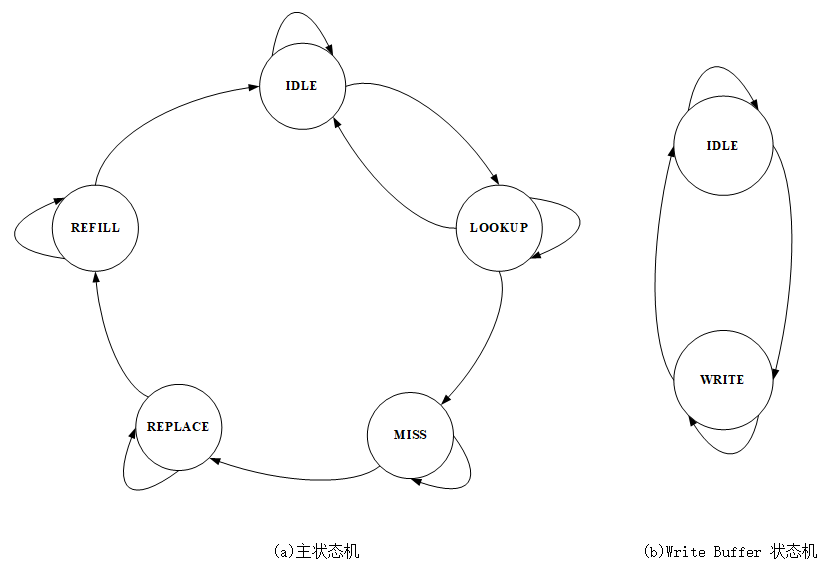
\includegraphics[width=1\linewidth]{assets/09/cache_fsm.png}
  \caption{Cache模块主状态机状态转移图}
  \label{fig:cache-fsm}
\end{figure}

Write Buffer状态机共包括2个状态，见图\ref{fig:cache-fsm}b。

\begin{itemize}
\tightlist
\item
  \textbf{IDLE}：Write Buffer当前没有待写的数据。
\item
  \textbf{WRITE}：将待写数据写入到Cache中。在主状态机处于LOOKUP状态且发现Store操作命中Cache时，触发Write Buffer状态机进入WRITE状态，同时Write Buffer会寄存Store要写入的Index、路号、offset、写使能（写32位数据里的哪些字节）和写数据。
\end{itemize}

以下是主状态机各状态之间的转换条件的详细说明：

\begin{enumerate}
\def\labelenumi{\arabic{enumi}.}
\tightlist
\item
  \textbf{IDLE}：

  \begin{itemize}
  \tightlist
  \item
    \textbf{IDLE → IDLE}：在这一时钟周期内，流水线没有新的Cache访问请求，或者有请求但因与Hit Write冲突而无法被Cache接收。
  \item
    \textbf{IDLE → LOOKUP}：在这一时钟周期内，Cache接收到了流水线发来的一个新的Cache访问请求（必定与Hit Write无冲突）。
  \end{itemize}
\item
  \textbf{LOOKUP}：

  \begin{itemize}
  \tightlist
  \item
    \textbf{LOOKUP → IDLE}：当前处理的操作是Cache命中，且在这一时钟周期内流水线没有新的Cache访问请求，或者有请求但因与Hit Write冲突而无法被Cache接收。
  \item
    \textbf{LOOKUP → LOOKUP}：当前处理的操作是Cache命中，且在这一时钟周期内Cache接收到了流水线发来的一个新的Cache访问请求（必定与Hit Write无冲突）。
  \item
    \textbf{LOOKUP → MISS}：当前处理的操作是Cache缺失。
  \end{itemize}
\item
  \textbf{MISS}：

  \begin{itemize}
  \tightlist
  \item
    \textbf{MISS → MISS}：AXI总线接口模块反馈wr\_rdy为0（注意，wr\_rdy应当先于wr\_req置上）。
  \item
    \textbf{MISS → REPLACE}：AXI总线接口模块反馈wr\_rdy为1（表示AXI总线内部16字节写缓存为空，可以接收wr\_req）。当wr\_rdy为1时，对Cache发起替换的读请求，并转到REPLACE状态。
  \end{itemize}
\item
  \textbf{REPLACE}：

  \begin{itemize}
  \tightlist
  \item
    \textbf{REPLACE → REPLACE}：AXI总线接口模块反馈rd\_rdy为0。刚进入REPLACE的第一时钟周期，会得到被替换的Cache行数据，并发起wr\_req送到AXI总线接口。由于wr\_rdy为1，故wr\_req一定会被接收。同时，对AXI总线发起缺失Cache的读请求。
  \item
    \textbf{REPLACE → REFILL}：AXI总线接口模块反馈rd\_rdy为1，表示对AXI总线发起的缺失Cache的读请求将被接收。
  \end{itemize}
\item
  \textbf{REFILL}：

  \begin{itemize}
  \tightlist
  \item
    \textbf{REFILL → REFILL}：缺失Cache行的最后一个32位数据（ret\_valid=1 \&\& ret\_last=1）尚未返回。
  \item
    \textbf{REFILL → IDLE}：缺失Cache行的最后一个32位数据（ret\_valid=1 \&\& ret\_last=1）从AXI总线接口模块返回。
  \end{itemize}
\end{enumerate}

以下是Write Buffer状态机各状态之间的转换条件的详细说明：

\begin{enumerate}
\def\labelenumi{\arabic{enumi}.}
\tightlist
\item
  \textbf{IDLE}：

  \begin{itemize}
  \tightlist
  \item
    \textbf{IDLE → IDLE}：在这一时钟周期内，Write Buffer没有待写的数据，并且主状态机没有新的Hit Write。
  \item
    \textbf{IDLE → WRITE}：在这一时钟周期内，Write Buffer没有待写的数据，并且主状态机发现新的Hit Write（主状态机处于LOOKUP状态且发现Store操作命中Cache）。
  \end{itemize}
\item
  \textbf{WRITE}：

  \begin{itemize}
  \tightlist
  \item
    \textbf{WRITE → WRITE}：在这一时钟周期内，Write Buffer有待写的数据，并且主状态机发现新的Hit Write。
  \item
    \textbf{WRITE → IDLE}：在这一时钟周期内，Write Buffer有待写的数据，并且主状态机没有新的Hit Write。
  \end{itemize}
\end{enumerate}

在主状态机的状态转换过程中，多次提到``与Hit Write有/无冲突''，这里的冲突分为两种情况：

\begin{enumerate}
\def\labelenumi{\arabic{enumi}.}
\item
  \textbf{主状态机处于LOOKUP状态且发现Store操作命中Cache}：此时，如果流水线发来一个新的Load类的Cache访问请求，并且该Load请求与LOOKUP状态的Store请求地址存在写后读相关性，即产生``与Hit Write冲突''。
\item
  \textbf{Write Buffer状态机处于WRITE状态}：即正在将待写数据写入Cache中，如果此时流水线发来一个新的Load类的Cache访问请求，并且该Load请求与Write Buffer中的待写请求的地址重叠。这里的``地址重叠''指的是Load请求地址的{[}3:2{]}与Store请求地址的{[}3:2{]}相等。
\end{enumerate}

以上两种情况都视为``与Hit Write冲突''。尽管对于第一种情况，可以采用``Write Buffer前递给LOOKUP''的方法解决，而不阻塞主状态机的转换，但为了简化，我们推荐采用阻塞方式处理。然而，第二种情况只能通过阻塞方式解决，即阻塞主状态机的转换。这种方法牺牲了一定的性能，但简化了设计。

在主状态机``LOOKUP → LOOKUP''的转换中，应注意避免引入RAM输出端到RAM输入端的路径。具体而言，主状态机发现一个命中的Cache访问并接收到一个新的Cache访问请求时，应避免使用命中信息（来自RAM读出的Tag比较）控制新的RAM的读使能。我们的解决方案是，无论LOOKUP状态的请求是否命中Cache，在控制``Hit Write冲突''和新的RAM使能生成时都视为命中考虑。即使最终发现不命中，也不会导致错误。

在主状态机``MISS → REPLACE''的转换过程中，当处于MISS状态时，我们确保AXI总线接口可以接收被替换Cache行的数据，同时对Cache RAM发起替换Cache行的读请求。下一拍（REPLACE状态）中，获得被替换的Cache行数据并将其发送到AXI总线接口模块（此时一定可以被接收）。同时，我们可以对AXI总线发起缺失Cache行的读请求。这种设计通过牺牲一定的性能来降低Cache模块和AXI总线接口模块在读返回路径上的握手复杂性，实现了无条件地将总线接口模块返回的数据直接写入Cache中。

需要提醒的是，对于ICache，可以将wr\_rdy恒设为1（此时MISS状态只会持续一拍），因为ICache不会真正发出wr\_req。

\subsubsection{表的片选和写使能}\label{sec:09-cache-017}

下表展示了Cache片选和写使能的逻辑：

\begin{longtable}[]{@{}
  >{\raggedright\arraybackslash}p{(\linewidth - 10\tabcolsep) * \real{0.0818}}
  >{\raggedright\arraybackslash}p{(\linewidth - 10\tabcolsep) * \real{0.0545}}
  >{\raggedright\arraybackslash}p{(\linewidth - 10\tabcolsep) * \real{0.1545}}
  >{\raggedright\arraybackslash}p{(\linewidth - 10\tabcolsep) * \real{0.3455}}
  >{\raggedright\arraybackslash}p{(\linewidth - 10\tabcolsep) * \real{0.1818}}
  >{\raggedright\arraybackslash}p{(\linewidth - 10\tabcolsep) * \real{0.1818}}@{}}
\toprule\noalign{}
\begin{minipage}[b]{\linewidth}\raggedright
Cache表项
\end{minipage} & \begin{minipage}[b]{\linewidth}\raggedright
\end{minipage} & \begin{minipage}[b]{\linewidth}\raggedright
Look Up
\end{minipage} & \begin{minipage}[b]{\linewidth}\raggedright
Hit Write
\end{minipage} & \begin{minipage}[b]{\linewidth}\raggedright
Replace
\end{minipage} & \begin{minipage}[b]{\linewidth}\raggedright
Refill
\end{minipage} \\
\midrule\noalign{}
\endhead
\bottomrule\noalign{}
\endlastfoot
\{Tag，V\} & 片选 & 2路 & - & & 替换那一路 \\
& 写使能 & 2路 & - & & 替换那一路 \\
D & 片选 & - & Write Buffer记录的那一路 & 替换那一路 & 替换那一路 \\
& 写使能 & - & Write Buffer记录的那一路 & - & 替换那一路 \\
Data & 片选 & 2路，请求所在Bank & Write Buffer记录的那一路，请求所在Bank & 替换那一路，所有Bank & 替换那一路，所有Bank \\
& 写使能 & - & Write Buffer记录的那一路，请求所在Bank & - & 替换那一路，所有Bank \\
\end{longtable}

\subsubsection{模块接口输出的控制相关信号}\label{sec:09-cache-018}

以下是对模块接口输出的控制相关信号置1条件的分析：

\textbf{流水线方向的 \texttt{addr\_ok} 信号}

\begin{itemize}
\tightlist
\item
  Cache主状态机处于 \texttt{IDLE} 状态。
\item
  或者，Cache主状态机处于 \texttt{LOOKUP} 状态，并将进行 \texttt{LOOKUP\ →\ LOOKUP} 的转换，具体包括：

  \begin{itemize}
  \tightlist
  \item
    \texttt{LOOKUP} 发现Cache命中，流水线发送来的新的Cache请求是写操作；
  \item
    \texttt{LOOKUP} 发现Cache命中，且新的Cache请求是读操作且无``Hit Write冲突''。
  \end{itemize}
\end{itemize}

\textbf{流水线方向的 \texttt{data\_ok} 信号}

\begin{itemize}
\tightlist
\item
  Cache当前状态为 \texttt{LOOKUP} 且Cache命中。
\item
  或者，Cache当前状态为 \texttt{LOOKUP} 且处理的是写操作。
\item
  或者，Cache当前状态为 \texttt{REFILL} 且 \texttt{ret\_valid=1}，同时Miss Buffer中记录的返回字个数与Cache缺失地址的 \texttt{{[}3:2{]}} 相等。
\end{itemize}

\textbf{AXI接口方向的 \texttt{rd\_req} 信号}

\begin{itemize}
\tightlist
\item
  当Cache模块状态机处于 \texttt{REPLACE} 状态时，组合逻辑将 \texttt{rd\_req} 置为1。在非 \texttt{REPLACE} 状态时，\texttt{rd\_req} 自然为0。
\end{itemize}

\textbf{AXI接口方向的 \texttt{wr\_req} 信号}

\begin{itemize}
\tightlist
\item
  设置一个触发器，复位期间清0。当Cache模块状态机从 \texttt{MISS} 转换到 \texttt{REPLACE} 状态时，将其置1。随后，当 \texttt{wr\_rdy} 为1时，将其从1清为0。
\end{itemize}

\subsection{Cache的硬件初始化问题}\label{sec:09-cache-019}

在LoongArch精简版指令集中，Cache可以通过软件进行初始化。在处理器复位结束后，CSR.CRMD的DATF和DMTM域都为0，此时取指和访存都是强序非缓存的，软件可以使用CACOP指令将Cache的Tag部分置为0。

在我们的实践工作中，考虑到实现工作量和理解上的复杂度，一般的我们将CACHE指令的实现放在了Cache实现的最后一个阶段。这引发了一个问题：在尚未实现CACOP指令的情况下，如何在上板验证时确保Cache已初始化。

Cache初始化至少要确保Cache中每一项的Tag、V和D的状态置为确定的无效值。由于Tag和V信息都存放在RAM中，因此解决方案是设计一个小型硬件电路，将存放Cache Tag和V信息的RAM的每一行写成全0值。还有一个偷懒的方法：利用实验中采用FPGA 硬件平台这一特点来简化Cache硬件初始化的实现。读者可以在生成Cache所用的RAM的时候，选择将RAM初始化成全0。

\section{Cache性能分析与优化}\label{sec:09-cache-020}

\textbf{Cache性能分析关键指标}

\begin{enumerate}
\def\labelenumi{\arabic{enumi}.}
\item
  \textbf{命中时的访问延迟（Hit Latency）}：命中时的访问延迟是指当Cache命中时，从发出请求到数据返回所需的时间。这一指标通常反映了Cache访问速度的快慢。理想情况下，命中时的访问延迟应该尽可能低，以确保快速的数据访问。
\item
  \textbf{失效时的访问延迟（Miss Latency）}：失效时的访问延迟是指当Cache未命中（Cache Miss）时，从发出请求到数据返回所需的时间。这一时间包括从主存储器或下一级Cache中获取数据并将其载入Cache的过程。失效时的访问延迟通常比命中时的访问延迟要高得多，因为涉及到更长的路径和更高的访问成本。
\item
  \textbf{失效时对后续访问的影响（Miss Penalty）}：失效时对后续访问的影响是指一次Cache失效对后续访问造成的额外延迟。这不仅包括获取所需数据的时间，还可能包括在载入新数据时将旧数据写回主存储器的时间。高失效率会导致频繁的Cache Miss，从而显著降低系统的整体性能。
\end{enumerate}

\textbf{可能的优化方向}

\begin{enumerate}
\def\labelenumi{\arabic{enumi}.}
\item
  \textbf{增大Cache容量}
  增大Cache容量可以减少Cache Miss的发生几率，从而降低失效时的访问延迟和对后续访问的影响。然而，增大容量也会增加Cache的物理尺寸和成本，并可能导致访问延迟增加。
\item
  \textbf{提高Cache的相联度}
  提高Cache的相联度（Associativity）可以减少冲突Miss的发生。全相联Cache的性能最好，但实现复杂度和成本较高。可以采用较高相联度的组相联Cache作为折中方案。
\item
  \textbf{采用多级Cache架构}
  现代处理器通常采用多级Cache（L1、L2、L3等）架构。较小的L1 Cache提供低延迟访问，而较大的L2、L3 Cache提供更大的存储容量。多级Cache架构可以在不同层次上优化访问延迟和Miss率。
\item
  \textbf{使用预取（Prefetching）技术}
  预取技术通过在实际访问前提前加载数据到Cache中来减少Miss率。预取可以是硬件预取或软件预取，但需要平衡预取的准确性和额外的带宽消耗。
\item
  \textbf{优化Cache替换算法}
  采用更智能的替换算法（如LRU、LFU等）可以减少不必要的数据替换，提高命中率。替换算法的选择对Cache性能有重要影响。
\item
  \textbf{减少Cache一致性开销}
  在多核处理器中，Cache一致性协议（如MESI、MOESI）用于确保各核Cache中的数据一致性。优化一致性协议或减少一致性开销可以提高Cache性能。
\end{enumerate}

\section{Cache集成到CPU中}\label{sec:09-cache-021}

事实上这部分内容在\textbf{Cache模块功能边界划分}部分已经给出了实现方案，按照接口定义将Cache对接进流水线即可。为避免读者陷入工程细节，本条主要在宏观层面上给出整体的实现思路

\textbf{命中情况下的适配}

当Cache命中时，数据可以在一个时钟周期内从Cache中获取（尽管一个完整的访存过程会经历两个以上周期，但是流水线技术有效的掩盖了这个问题，即整体看来，访存流水线每周期可处理一条访存指令），这对于流水线来说是理想的情况。在经典的五级RISC流水线中（取指、译码、执行、存储访问、写回），Cache命中意味着存储访问阶段（MEM）能够在一个周期内完成，从而不影响流水线的顺利进行。这样可以保持流水线的高效运行，减少等待时间和潜在的流水线停顿。

\textbf{缺失情况下的适配}

当Cache缺失（Cache Miss）时，CPU流水线必须等待从主存或更低级的存储器获取数据，这会导致流水线停顿。具体而言，缺失会触发一个存储访问异常，Cache一般使用状态机处理数据缺失，需要多个周期来完成数据的读取。这种情况，顺序执行的处理器通常会暂停流水线以保持流水线同步，但这也意味着处理器效率下降。为了应对这一问题，现代处理器通常会使用非阻塞缓存（Non-blocking Cache）和乱序执行（Out-of-order Execution）来减少Cache Miss对流水线的影响。

\textbf{Uncache访问的处理}

Uncache访问（非缓存访问）通常用于访问那些不适合缓存的数据，比如I/O设备的寄存器。这类访问直接与主存或I/O设备交互，不经过Cache，因此延迟较高。为了适应这类访问，CPU通常设计专门的路径和控制逻辑，以确保数据的正确性和一致性。当然为了方便实现也可以复用Cache的访存状态机，即强制让Uncache访问指令发生Cache缺失，从而启动Cache的恢复流程，利用Cache在该流程中的写回和读取逻辑完成Uncache访问功能。

\section{支持Cache处理器的性能调优}\label{sec:09-cache-022}

在确定架构完成Cache的集成后，在最顶层宏观的方法学视角上处理器已经没有较大的优化空间了。但在具体的实践中，即使不改变整体架构，处理器的性能往往还有较大的提升空间，这主要是因为我们实现的处理器很可能存在``性能BUG''。\textbf{解决这些性能BUG的过程就是性能调优的过程。}

在面对复杂系统的性能优化时，我们经常需要做出许多决策，例如确定哪些部分值得优化、选择哪种优化策略、预测可能的收益以及评估这些策略的成本。显然，如果巨大的努力仅带来微小的性能提升，这并不符合我们的预期。因此，相较于盲目编程，我们更需要一套科学的方法论来指导我们解答以下关键问题：

\begin{enumerate}
\def\labelenumi{\arabic{enumi}.}
\tightlist
\item
  \textbf{评估当前性能}：通过定量的指标，如执行时间和资源利用率，来全面了解系统的现状。
\item
  \textbf{识别性能瓶颈}：通过性能分析工具，如性能分析器和日志分析，来确定影响系统效率的关键因素。
\item
  \textbf{选择适当的优化策略}：根据瓶颈的性质，决定采取算法优化、资源增配、系统配置调整等方法。
\item
  \textbf{评估优化效果}：实施优化后，再次进行性能评估，并与优化前的性能数据进行对比，以验证优化的有效性是否符合预期。
\end{enumerate}

\subsection{性能评估}\label{sec:09-cache-023}

在讨论性能优化之前，首先必须确立系统当前的运行状态。因此，我们需要一个定量的性能衡量指标，而不仅仅依赖主观感觉来判断系统的运行效果。通过这种定量指标，我们能够客观评估现有系统的性能，这是性能优化的初步步骤。

在通常的理解中，``高性能''往往意味着``运行速度快''。因此，一个直观的性能衡量指标是程序的执行时间。简而言之，评估一个系统的性能就是测量程序在该系统上的执行时间。通过这种方法，我们可以准确地识别出性能瓶颈，从而有针对性地进行优化。

在选择基准程序时，关键在于选取能够代表实际应用场景的程序集。这些程序应当能够反映出在特定优化技术下，预期性能提升与实际应用场景中性能提升的一致趋势。

\subsubsection{基准测试程序}\label{sec:09-cache-024}

不同的应用场景可能需要不同的代表性程序，从而形成各自的benchmark。例如，Linpack被用于代表超级计算场景，MLPerf针对的是机器学习训练场景，CloudSuite用于云计算场景，而Embench则专注于嵌入式场景。对于通用计算场景，最著名的benchmark是SPEC CPU，由Standard Performance Evaluation Corporation (SPEC) 组织发布，该组织旨在建立和维护用于评估计算机系统性能的标准。

SPEC CPU 2006是一个广泛使用的benchmark，包括整数和浮点测试，涵盖了多种应用程序，例如：

\begin{itemize}
\tightlist
\item
  \textbf{整数测试}：

  \begin{itemize}
  \tightlist
  \item
    \texttt{400.perlbench}：利用Perl语言检测垃圾邮件
  \item
    \texttt{401.bzip2}：bzip压缩算法
  \item
    \texttt{403.gcc}：gcc编译器
  \item
    \texttt{429.mcf}：针对大型公共交通中单站车辆调度的组合优化问题
  \item
    \texttt{445.gobmk}：围棋AI搜索问题
  \item
    \texttt{456.hmmer}：使用隐马尔可夫模型进行基因序列搜索
  \item
    \texttt{458.sjeng}：国际象棋AI搜索问题
  \item
    \texttt{462.libquantum}：量子计算模拟素数分解
  \item
    \texttt{464.h264ref}：对YUV格式源文件进行H.264视频编码
  \item
    \texttt{471.omnetpp}：大型CSMA/CD协议以太网模拟
  \item
    \texttt{473.astar}：使用A*算法进行路径寻找
  \item
    \texttt{483.xalancbmk}：XML到HTML的格式转换
  \end{itemize}
\item
  \textbf{浮点测试}：

  \begin{itemize}
  \tightlist
  \item
    覆盖流体力学、量子化学、生物分子研究、有限元分析、线性规划、影像光线追踪、计算电磁学、天气预报、语音识别等领域。
  \end{itemize}
\end{itemize}

随着技术的演进，benchmark也需要不断更新以反映新的应用趋势。例如，SPEC CPU 2017版本引入了一些新程序，如生物医学成像、3D渲染和动画、采用蒙特卡罗树搜索的人工智能围棋程序，这些新加入的测试项目大大提高了benchmark的时代相关性和实用性。通过这些更新，SPEC帮助研究人员和工程师准确评估和优化不断变化的技术环境中的系统性能。

但对于面向教学的CPU设计实践来说, SPEC CPU的程序有点过于真实了: 一方面它们的规模很大, 即使在x86真机中也需要花费小时的时间来运行; 另一方面它们需要运行在Linux环境中, 这意味着我们首先需要设计一个能正确启动Linux的CPU, 然后才能运行SPEC CPU这个benchmark。对于我们的应用场景来说，传统的Dhrystone与CoreMark测试程序已经足够了。

\textbf{Dhrystone}

Dhrystone是一种经典的CPU性能基准测试程序，主要用于评估整数运算的性能。它以其简单、便于移植和使用广泛而著称。Dhrystone使用合成的程序来模拟常见的计算工作负载，通过测量在特定时间内执行的Dhrystone操作数（DMIPS），来评估CPU的性能。然而，Dhrystone的一个主要缺陷是容易被编译器优化，导致结果更多反映了编译器的优化能力而非CPU的实际性能。

\textbf{CoreMark}

CoreMark是由嵌入式微处理器基准测试联盟（EEMBC）开发的一种现代CPU性能测试程序，旨在替代Dhrystone。它通过实现四种常见算法（链表处理、矩阵操作、状态机和循环冗余校验）来测量CPU核心的性能。CoreMark的设计避免了编译器的过度优化问题，提供了一种更为公平和一致的性能评估方法。

\subsection{性能瓶颈}\label{sec:09-cache-025}

要准确地评估和优化系统性能，单一的运行时间数据确实不足以全面反映系统性能的各个方面。因此，更细致地分析程序的运行时间，将其分解成三个基本因素：程序指令数量、每条指令的执行周期数（CPI），以及每个周期的时间，是一种有效的方法。这种分解不仅有助于精确定位性能瓶颈，还能为性能优化提供明确的方向。

\[
perf = \frac{time}{prog} = \frac{inst}{prog} \times \frac{cycle}{inst} \times \frac{time}{cycle}
\]

其中:

\begin{itemize}
\tightlist
\item
  \(perf\) 表示程序性能
\item
  \(time\) 表示程序执行总时间
\item
  \(prog\) 表示程序\\
\item
  \(inst\) 表示指令
\item
  \(cycle\) 表示处理器时钟周期
\end{itemize}

这个公式描述了程序性能与指令数、指令周期和时钟周期之间的关系。它表明程序性能取决于这三个因素的乘积。

获取性能指标：

\begin{itemize}
\tightlist
\item
  \textbf{动态指令数}：在仿真环境中直接统计。
\item
  \textbf{周期数和IPC}：通过仿真数据和周期精确计数来计算。（chiplab仿真环境的输出提供了这个数据）
\item
  \textbf{频率}：从电路综合报告中获取。
\end{itemize}

以下是详细的性能优化策略：

\begin{enumerate}
\def\labelenumi{\arabic{enumi}.}
\tightlist
\item
  \textbf{减少程序执行的动态指令数}

  \begin{itemize}
  \tightlist
  \item
    \textbf{优化算法和程序设计}：选择更高效的算法和数据结构，减少必要的计算步骤和资源消耗。
  \item
    \textbf{编译器优化}：利用编译器的高级优化选项，如 \texttt{-O3} 或 \texttt{-Ofast}。特定的编译器选项可以进一步降低动态指令数，从而提高性能。
  \item
    \textbf{使用复杂指令集（CISC）或自定义指令}：采用复杂的指令或向处理器添加专用硬件加速指令，有效减少总指令数。
  \end{itemize}
\item
  \textbf{降低每条指令的周期数（提升IPC）}

  \begin{itemize}
  \tightlist
  \item
    \textbf{微结构优化}：设计高效的处理器微结构，如超标量执行、流水线和乱序执行，使每个时钟周期内执行更多指令。
  \item
    \textbf{并行处理技术}：通过多线程和多核技术提高并行处理能力，增加每周期执行的指令数。
  \end{itemize}
\item
  \textbf{减少每个周期的时间（提升频率）}

  \begin{itemize}
  \tightlist
  \item
    \textbf{前端设计优化}：优化处理器逻辑设计，减少关键路径的逻辑延迟，允许更高的时钟频率。
  \item
    \textbf{后端设计优化}：改进物理设计，如走线优化和布局调整，减少信号传播延迟，提升频率。
  \end{itemize}
\end{enumerate}

\subsection{缓存优化}\label{sec:09-cache-026}

\subsubsection{缓存技术与性能评价}\label{sec:09-cache-027}

缓存技术主要用于提升访存效率，因此我们应通过访存相关的指标来评价缓存的性能表现。通常，我们使用平均内存访问时间（AMAT, Average Memory Access Time）来评估缓存的性能。假设缓存的命中率为 \(p\)，则 AMAT 的计算公式如下：

\[
AMAT = access\_time + (1 - p) \times miss\_penalty
\]
其中，access\_time 是缓存的访问时间，即从缓存接收到访存请求到得出命中结果所需的时间；miss\_penalty 是缓存缺失时的代价，即访问 DRAM 的时间。

这一等式为优化缓存性能提供了指导方向：减少访问时间（access\_time）、提高命中率（p）或减少缺失代价（miss\_penalty）。在当前的 NPC（Non-Predictable Cache）中，访问时间在架构设计上的优化空间有限，更多地受具体实现的影响，如周期数和关键路径。因此，我们将重点讨论命中率和缺失代价的优化策略。

\subsubsection{提升命中率}\label{sec:09-cache-028}

为了提升缓存的命中率，即降低缺失率，我们首先需要了解缓存缺失的原因。

\textbf{缓存缺失的3C模型}

计算机科学家Mark Hill在其1987年的博士论文中提出了3C模型，用以描述缓存缺失的三种类型：

\begin{enumerate}
\def\labelenumi{\arabic{enumi}.}
\tightlist
\item
  \textbf{强制缺失（Compulsory Miss）}：定义为在一个容量无限大的缓存中发生的缺失，通常在第一次访问一个数据块时发生。
\item
  \textbf{容量缺失（Capacity Miss）}：定义为由于缓存容量不足而无法避免的缺失，表现为缓存无法容纳所有需要访问的数据。
\item
  \textbf{冲突缺失（Conflict Miss）}：定义为由于缓存映射冲突引起的缺失，表现为多个数据块之间相互替换导致的缺失。
\end{enumerate}

通过理解3C模型，我们可以针对每种类型的缺失提出相应的解决方案，以降低缺失率。

\textbf{降低强制缺失}

\begin{enumerate}
\def\labelenumi{\arabic{enumi}.}
\tightlist
\item
  \textbf{预取机制}：为了降低强制缺失，原则上需要在访问一个数据块之前就将其读入缓存中。这可以通过添加预取（prefetch）机制实现。
\item
  \textbf{强制缺失占比低}：理论上，强制缺失只发生在首次访问某数据块时，因此在高频访问场景下，强制缺失的占比较低。对此感兴趣的读者可以查阅更多关于预取的资料。
\end{enumerate}

\textbf{降低容量缺失}

\begin{enumerate}
\def\labelenumi{\arabic{enumi}.}
\tightlist
\item
  \textbf{扩大缓存容量}：根据定义，降低容量缺失的唯一方法是扩大缓存容量，以更好地利用时间局部性。
\item
  \textbf{综合考虑因素}：缓存容量并非越大越好。一方面，较大的缓存容量意味着较大的芯片面积，从而增加流片成本；另一方面，较大的存储阵列会增加访问延迟，降低缓存性能。因此，在实际项目中，需要综合考虑各方面因素进行权衡，不能一味追求更大的缓存容量。
\end{enumerate}

\textbf{降低冲突缺失}

\begin{enumerate}
\def\labelenumi{\arabic{enumi}.}
\tightlist
\item
  \textbf{减少替换情况}：为了降低冲突缺失，需要减少多个缓存块之间相互替换的情况。
\item
  \textbf{全相联缓存}：采用全相联（fully-associative）的缓存组织方式是一种极端方法，允许数据块存放到任意缓存块中。然而，这种方式需要更多的存储开销和比较器，通常仅在缓存块数量较少的情况下使用。
\item
  \textbf{组相联缓存}：组相联（set-associative）是直接映射和全相联的折中方案。其思想是将所有缓存块分组，在组间通过直接映射方式选出一个组，然后在组内通过全相联方式选出一个缓存块。例如，若每组有w个缓存块，则称为w路组相联（w-way set-associative）。现代CPU通常采用8或16路组相联。
\end{enumerate}

\textbf{块大小的选择}

\begin{enumerate}
\def\labelenumi{\arabic{enumi}.}
\tightlist
\item
  \textbf{降低tag存储开销}：较大的缓存块能够降低tag的存储开销，并捕捉更多的空间局部性，降低冲突缺失。
\item
  \textbf{权衡缺失代价}：较大的缓存块也会增加缺失代价，并在空间局部性不明显的情况下增加冲突缺失。具体的块大小选择需根据程序的空间局部性特征进行权衡。
\end{enumerate}

\subsubsection{优化缺失代价}\label{sec:09-cache-029}

当缓存发生缺失时，需要访问下一层存储层次，缺失代价即为该层存储的访问时间。降低缺失代价的技术有很多，本文将探讨其中一种：总线传输的突发访问。

\textbf{块大小和缺失代价}

当前的缓存设计中，下一层存储通常为SDRAM。为了进一步分析，我们将SDRAM的访问时间划分为以下四个阶段：

\begin{enumerate}
\def\labelenumi{\arabic{enumi}.}
\tightlist
\item
  \textbf{a}：AR通道握手，接收读请求。
\item
  \textbf{b}：状态机转移到READ状态，并向SDRAM发送READ命令。
\item
  \textbf{c}：SDRAM返回读数据。
\item
  \textbf{d}：R通道握手，返回读数据。
\end{enumerate}

假设总线的数据位宽为4字节，缓存块大小为16字节。如果采用4个独立的总线传输事务，则总开销为4(a + b + c + d)。

\textbf{总线的突发传输}

类似于SDRAM芯片，AXI总线也支持``突发传输''（burst transfer），即在一次总线传输事务中包含多次连续的数据传输。每次数据传输称为一个``节拍''（beat）。在AXI总线协议中，需要通过AR通道的\texttt{arburst}信号指示此次传输是否采用突发传输；如果是，还需要通过\texttt{arlen}信号指示此次突发传输的节拍数量。

当然，仅有总线协议的支持是不够的，还需要AXI的主设备（master）端发起突发传输事务，并且从设备（slave）端支持突发传输事务的处理。作为主设备端的icache，我们将发起突发传输事务的实验内容留给大家。另一方面，ysyxSoC提供的SDRAM控制器确实支持突发传输事务的处理，可以将上述四次总线传输包含在一次总线事务中，从而有效降低完整读出一个数据块的开销：

首先，通过突发传输，AR通道只需要进行一次握手，相比于传统方案，开销可节省\texttt{3a}。其次，SDRAM控制器可以将一次突发传输事务拆分成多个发往SDRAM芯片的READ命令。当SDRAM芯片返回一次读数据时，如果还有地址连续的READ命令，SDRAM控制器的状态机则直接转移到READ状态继续发送READ命令，与传统方案相比，开销可节省\texttt{3b}。最后，SDRAM控制器对R通道的回复可以与下一次READ命令的发送同时进行，从而将R通道握手的开销隐藏起来，与传统方案相比，开销可节省\texttt{3d}。

% 代码语言：BookText
\begin{CodeBlock}[language=BookText]
      a     b      c    d
    |---|-------|-----|---| <-------------------- 第1个节拍
                      |-----|---| <-------------- 第2个节拍
                            |-----|---| <-------- 第3个节拍
                                  |-----|---| <-- 第4个节拍
\end{CodeBlock}

综上，采用突发传输的开销为\texttt{a+b+4c+d}，相比传统方案，可以节省\texttt{3(a+b+d)}的开销。推广到一般情况，如果缓存块的大小是总线数据位宽的\texttt{n}倍，则采用突发传输可以节省\texttt{n(a+b+d)}的开销。虽然表面上看\texttt{a}、\texttt{b}和\texttt{d}的开销不大，但别忘了这是SDRAM控制器视角的开销，校准访存延迟后，对CPU来说可能节省数十甚至上百个周期的开销。

\subsubsection{设计空间探索方法总结}\label{sec:09-cache-030}

设计空间探索（Design Space Exploration, DSE）涉及选择一组适当的参数，以在给定资源下实现最佳性能。本文总结了一种有效的方法，通过降低统计精度以提高探索效率。

\textbf{1. 性能指标和评估}

我们关注的性能指标包括指令每周期（Instructions Per Cycle, IPC）、主频（Frequency）和面积（Area）。主频和面积可以通过快速硬件综合工具评估，而IPC通常需要运行完整的程序以获得准确数据。

\textbf{2. 平衡数据精度和仿真效率}

由于不同参数组合的数量庞大，如果每种组合都需要耗费大量时间来获取IPC，设计空间探索的效率将非常低。因此，需要在数据精度和仿真效率之间进行权衡。为提高效率，可以通过较低的开销来统计一个能体现IPC变化趋势的指标，而不是追求绝对精确的IPC值。

\textbf{3. 平均内存访问时间和总缺失时间}

调整缓存参数直接影响平均内存访问时间（Average Memory Access Time, AMAT）。假设CPU中其他部分的执行开销保持不变，根据AMAT定义，调整这些参数并不影响缓存访问时间。因此，重点关注程序在发生缓存缺失时的等待总时间，即总缺失时间（Total Miss Time, TMT）。TMT越小，每条指令访存所需的周期数越少，从而IPC越大。

\textbf{4. 缺失次数统计}

为低开销地统计TMT，从缺失次数和缺失代价两个方面入手：

\begin{itemize}
\item 缺失次数：缓存的访问次数在给定程序中是固定的。通过指令跟踪（itrace）输入缓存，模拟缓存的工作过程，统计缺失次数，无需完整仿真整个系统。
\item 生成PC序列：指令跟踪已经包含完整的指令流，只需要指令流的PC值，而不需要指令本身。因此，通过PC序列可以模拟缓存的缺失统计。
\item 元数据维护：缓存的缺失次数与访存内容无关，只需维护元数据即可统计出正确的缺失次数。
\end{itemize}


\textbf{5. 缓存功能模拟器}

设计一个简单的缓存功能模拟器（cachesim），接收指令流的PC序列，通过维护元数据统计缺失次数。指令流的PC序列可以通过指令模拟器快速生成。

\textbf{6. 缺失代价估算}

缓存功能模拟器不包含访存细节，无法准确获取缺失代价。根据前述讨论，只有缓存块大小影响缺失代价，因此可以通过统计出一个平均缺失代价，作为常数估算TMT。

通过以上方法，可以在设计空间探索中，以较低的开销获得反映IPC变化趋势的指标，从而提高探索效率。

\subsection{经典体系结构的四类优化方法}\label{sec:09-cache-031}

找到性能瓶颈后，我们可以考虑如何对其进行优化。在经典体系结构中，主要有以下四类优化方法：

\begin{enumerate}
\def\labelenumi{\arabic{enumi}.}
\tightlist
\item
  \textbf{局部性}： 局部性优化利用数据访问的性质提升指令和数据供给能力。代表性技术是缓存，通过缓存提高访问数据的速度，减少延迟。
\item
  \textbf{并行}： 并行优化通过多个实例同时工作，提升系统的整体处理能力。并行方法可以进一步细分为：

  \begin{itemize}
  \tightlist
  \item
    \textbf{指令级并行（ILP）}：通过同时执行多条指令来提高性能，相关技术包括流水线、多发射、VLIW（超长指令字）和乱序执行。
  \item
    \textbf{数据级并行（DLP）}：通过同时访问多个数据来提高性能，相关技术包括SIMD（单指令多数据流）和向量指令/向量机。
  \item
    \textbf{任务级并行（TLP）}：通过同时执行多个任务来提高性能，相关技术包括多线程、多核、多处理器和多进程；GPU属于SIMT（单指令多线程），是一种介于数据级并行和任务级并行之间的并行方法。
  \end{itemize}
\item
  \textbf{预测}： 预测优化在不确定正确选择时，先投机地执行一个选择，在后续检查选择是否正确。如果预测正确，能降低等待的延迟，从而获得性能收益。如果预测错误，需要通过额外的机制进行恢复。代表性技术包括分支预测和缓存预取。
\item
  \textbf{加速器}： 使用专门的硬件部件来执行特定任务，从而提升该任务的执行效率。例子包括：

  \begin{itemize}
  \tightlist
  \item
    \textbf{AI加速器}：对AI负载的计算过程进行加速，通常通过总线访问。
  \item
    \textbf{自定义扩展指令}：将加速器集成到CPU内部，通过新增的自定义扩展指令来访问。
  \item
    \textbf{乘除法器}：可以视为一类加速器，通过乘除法指令控制专门的乘除法硬件模块，加速乘除法的计算过程。
  \end{itemize}
\end{enumerate}
